\documentclass{xduugthesis}

\usepackage{minted}  % 渲染代码语法高亮,需要安装 Python 和 Python Pygments 包
\usepackage{booktabs}  % 绘制三线表
\usepackage{amsmath}  % \text{} command

\usepackage{tikz}

\xdusetup{
    style = { cjk-font = founder, latin-font = tac }, 
    % style = { cjk-font = fandol, latin-font = gyre }, % 这两个字体是通用字体,但是 fandol 字符少,gyre 不好看
    info = {
        student-id = {},
        class-id = {},
        title = {},
        department = {计算机科学与技术学院},
        major = {软件工程},
        author = {},
        supervisor = {},
        abstract = {chapters/00-abstract},
        abstract* = {chapters/00-abstract-en},
        keywords = {关键词1,关键词2,关键词3},
        keywords* = {Keyword1,Keyword2,Keyword3},
        acknowledgements = {chapters/05-acknowledgements},
        bib-resource = {references.bib},
        appendix = {chapters/06-appendix}
    }
}

\begin{document}

% 定义常用宏
\newcommand\sysname{Narwhal}  % \sysname 会被替换为 Narwhal

% 定义定理和推论环境
\newtheorem{theorem}{Theorem}[section]  % {命令名}{定理标题}[标号级别]
\newtheorem{lemma}{Lemma}[theorem]  % 引理
\newtheorem{proof}{Proof}  % 证明不需要标号

\chapter{引言}

这里是引言

\chapter{正文}

\section{Figure}

这是一张图片

\begin{figure}[ht]  % h: here, t: top
    \centering  % 居中显示
    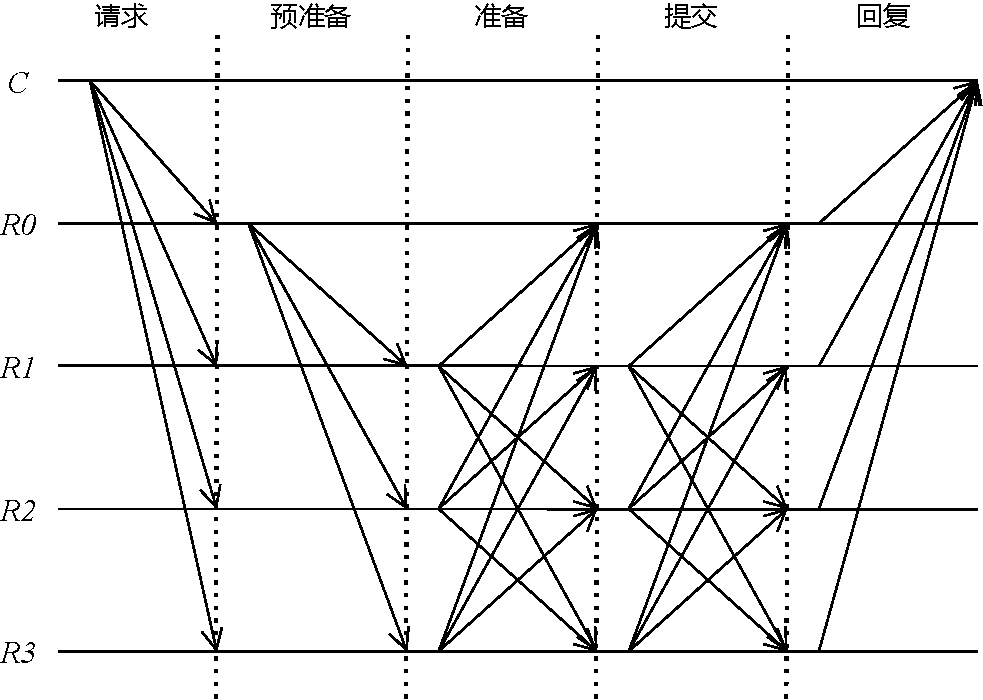
\includegraphics[width=0.85\columnwidth]{figures/pbft.pdf}  % 插入图片
    \caption{图片说明}
    \label{fig:dag}  % 引用标签
\end{figure}

这是图片的引用 \ref{fig:dag}

\section{Tabular}

这是一个表格

\begin{table}[ht]  % h: here, t: top
    \begin{center}
    % 一个字母代表一列
    \begin{tabular}{|c|cccc|}  % c: center, l: left, r: right
    \hline
      & 00 & 01 & 11 & 10\\
    \hline
    0 & $m_0$ & $m_1$ & $m_3$ & $m_2$\\
    1 & $m_4$ & $m_5$ & $m_7$ & $m_6$\\
    \hline
    \end{tabular}
    \end{center}
    \caption{表格说明} 
    \label{tab:1}  % 引用标签
\end{table}

这是一个三线表

\begin{table}[ht]
    % center 和 centering 的区别是 center 和上下文之间有垂直间隙
    % 而 centering 没有
    \centering
    \begin{tabular}{cccc}
    \toprule  % 第一道横线
    Item 1 & Item 2 & Item 3 & Item 4 \\
    \midrule  % 第二道横线 
    Data 1 & Data 2 & Data 3 & Data 4 \\
    Data 5 & Data 6 & Data 7 & Data 8 \\
    \bottomrule  % 第三道横线
    \end{tabular}
    \caption{表格说明}
    \label{tab:2}
\end{table}

\section{Citation}

上标引用All You Need is DAG\cite{keidar2021all}。

非上标引用All You Need is DAG\parencite{keidar2021all}
\section{Theorem}

% 需要在 macros.tex 中定义定理环境

这是一个定理

\begin{theorem}[YouTube]  % 定理名是可选的
    You should like and subscribe!
\end{theorem}

这是一个引理

\begin{lemma}
    And checkout Overleaf as well!
\end{lemma}

这是一个证明

\begin{proof}
    Left to the interested subscriber
\end{proof}

\section{List}

这是一个有序列表

\begin{enumerate}
    \item This is item 1
    \item This is item 2
\end{enumerate}

这是一个无序列表

\begin{itemize}
    \item This is an item.
    \item This is another item.
\end{itemize}

\section{Code}

这是一个围栏代码块

\usemintedstyle{trac}

\begin{minted}{python}

def main():
    print("Hello, world!")
    return 0

\end{minted}


\chapter{结论}

这里是结论
\chapter{结束语}

这里是结束语

\end{document}